%For printing? \documentclass[a4paper,10pt,twoside]{article}
\documentclass[a4paper,10pt]{article}

\usepackage{ucs}
\usepackage{caption}
\usepackage{pst-all}

\usepackage{xcolor}
\usepackage{fontenc}
\usepackage{graphicx}

\usepackage[dvips]{hyperref}
\usepackage[dcucite]{harvard}

\usepackage{wrapfig}

\usepackage{tikz}
\usetikzlibrary{calc,mindmap,backgrounds,arrows,shapes.multipart,fit}
\usepackage{pgf-umlcd}
\usepackage{scalefnt}


\renewcommand{\topfraction}{0.85}
\renewcommand{\textfraction}{0.1}
\renewcommand{\floatpagefraction}{0.75}

\title{Real-Time Interactive 3D Modelling with Commodity Hardware
\vspace{30pt}}
\author{Peter Coetzee\\Supervisor: Andrew Davison
\vspace{30pt}}
\date{June 2010}

\begin{document}
\maketitle

\vspace{50pt}

\begin{abstract}
A long-standing problem in Computer Vision has been recovery of scene geometry; in both controlled and (in many cases) arbitrary environments. With applications ranging from robot navigation to augmented reality in film and television, the process of taking a real-world object and representing it in 3D has enormous inherent value. Nevertheless, existing techniques all leave something to be desired; be it their cost, the limited range of their applicability, or their accuracy.

The theoretical approach outlined in this document aims to alleviate many of the aforementioned pitfalls of traditional methods, by utilising cheap commodity hardware for recognition, by creating a system that is robust in completely un-controlled environmental conditions, and by making use of both \textit{human} and \textit{machine} intelligence in the manners best suited to them.
\end{abstract}

\pagebreak
\tableofcontents
\pagebreak

\section{Motivation}
There are a deceptively large number of industries with an interest in producing accurate 3D models of objects in the real world. Engineers, for example, working on a CAD model of a product upgrade may want to scan the old product as a base template. The visual effects industry invests thousands of pounds in laser scans for every show they work on; it is critically important that ``digital doubles" (digital replications of human beings) are identical to the people they are based on, both for immersion and often for technical reasons too. It is not unusual for a VFX studio to take a live action scene and replace the actor with their digital double, so that (for example) shadows are cast correctly, or some particularly gruesome mutilation can occur (such as for Harvey Dent's character in the recent Dark Knight movie, seen in Figure~\ref{twoface}).

\begin{figure}[h]
  \begin{center}
    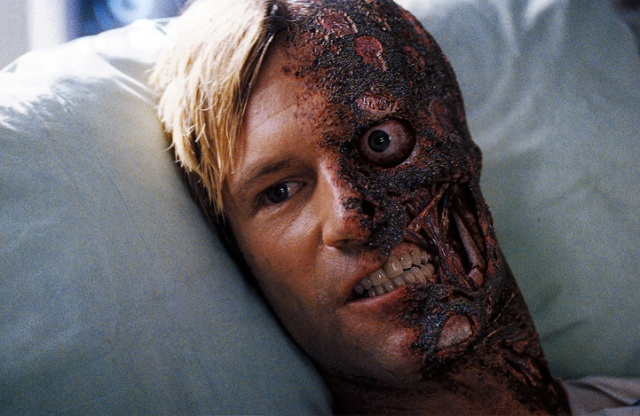
\includegraphics[width=340px]{twoface}
  \end{center}
  \vspace{-10pt}
  \caption{CGI Compositing: Digital Makeup for Harvey `Two-Face' Dent in The Dark Knight, \protect \copyright 2007 Warner Bros. Pictures}
  \label{twoface}
\end{figure}

Unless a studio owns the (typically expensive) equipment themselves, it can take weeks to get results back from 3rd party LIDAR scanning - if they had a means by which to create accurate models quickly and cheaply, they could do away with this expense altogether. In conversations with VFX professionals it emerges that the real challenge is to get an accurate \textit{proportional} reconstruction; artistic modelling can fill in as much detail as is desired, but to get the model in proportion a physical scan is required, by way of a foundation.

Furthermore, an increasing number of desktop applications are being produced to allow users to add models to their favourite games and social experiences; from Second Life to Quake, more people are learning 3D modelling and texture artistry. If they had a way of getting real-life objects into their games without having to undergo the horrifically steep learning curve of tools like Autodesk Maya or Mudbox, they would jump on the opportunity.

\section{Background}

As mentioned above, there are a variety of approaches to this well-studied problem available today. These solutions are typically selected to fit the particular use-case for the 3D model; their various strengths and weaknesses tend to recommend one over the other in any given situation.


\subsection{LIDAR}

\begin{wrapfigure}{r}{80pt}
  \vspace{-30pt}
  \begin{center}
    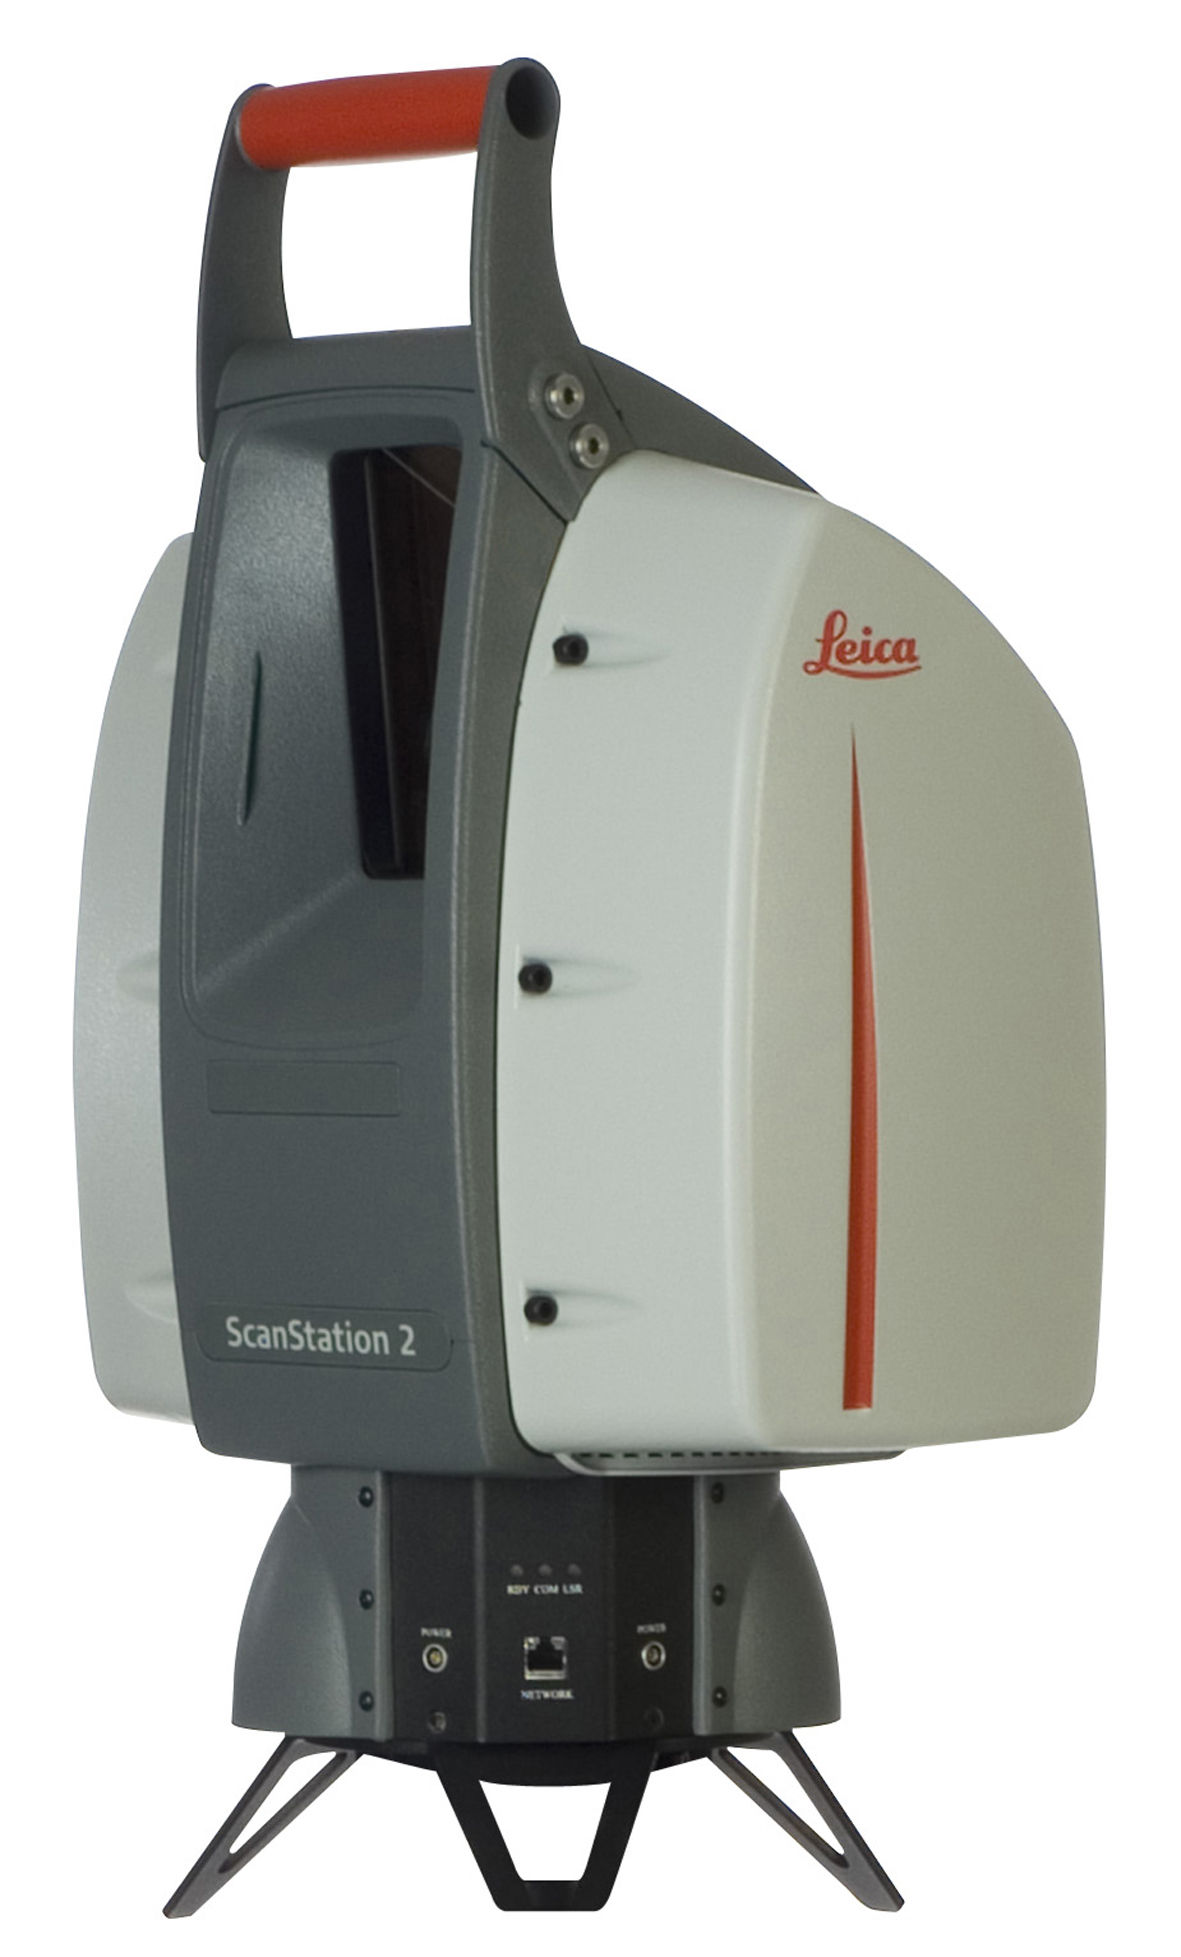
\includegraphics[width=80pt]{scanstation}
  \end{center}
  \caption{A Leica LIDAR Scanner}
  \label{scanstation}
  \vspace{-10pt}
\end{wrapfigure}

One common system used in the visual effects industry is LIDAR capture \cite**{lidar}, in which a scanning laser is used to trace the distance between it and the target object.
The object (or the scanner) is typically rotated during this process in order to generate a dense, 360$^\circ$ point-cloud representation of the scanned object. This technique, while expensive, is applicable in a variety of scenarios; from high-resolution facial capture through to large scale airborne ground topology scanning. This process requires little user intervention, and generates a large amount of data relatively quickly. However, much post-processing of this data is typically required; as it is a slightly noisy point-cloud, it must be cleaned up before it can be used in any real application. Furthermore, this cloud of points is not, by itself, geometry; it is more a set of candidate vertices for geometry, many of which will be discarded as they lie on surfaces. As a result, steps must be taken to generate surfaces in 3D which will fit these points.

\subsection{Automated Vision-Based Reconstruction}

One set of potentially valuable solutions which have received a lot of research attention recently are those around computer vision based systems. These show promise, in that they are based on much simpler hardware than LIDAR systems, instead focussing their complexity in intelligent software to analyse full colour imagery and extract the geometry from it. They are often based on using either a stereo camera, and thus using the fixed separation of the lenses to recover depth data, or augmenting a single lens with a laser rangefinder (a sort of vision-augmented LIDAR system). The details of implementation of such systems varies wildly. On one end of the scale, Photosynth \cite**{photosynth} employs heavy vision processing on still photographs of a given scene (potentially taken with different cameras, lenses, and in varying lighting conditions) and constructs a 3D montage of these images in order to give the effect of a textured 3D model. As part of this process, it actually constructs a coloured point cloud (as seen in Figure~\ref{photosynthcloud}), in much the same fashion as a LIDAR scan, and matches these points probabilistically to features in the set of input images. Work has been done \cite**{multistereo} on a similar approach with the goal of constructing arbitrary 3D surfaces, rather than just interpolation of the views presented by a finite set of images.

\begin{figure}
  \vspace{-35pt}
  \begin{center}
    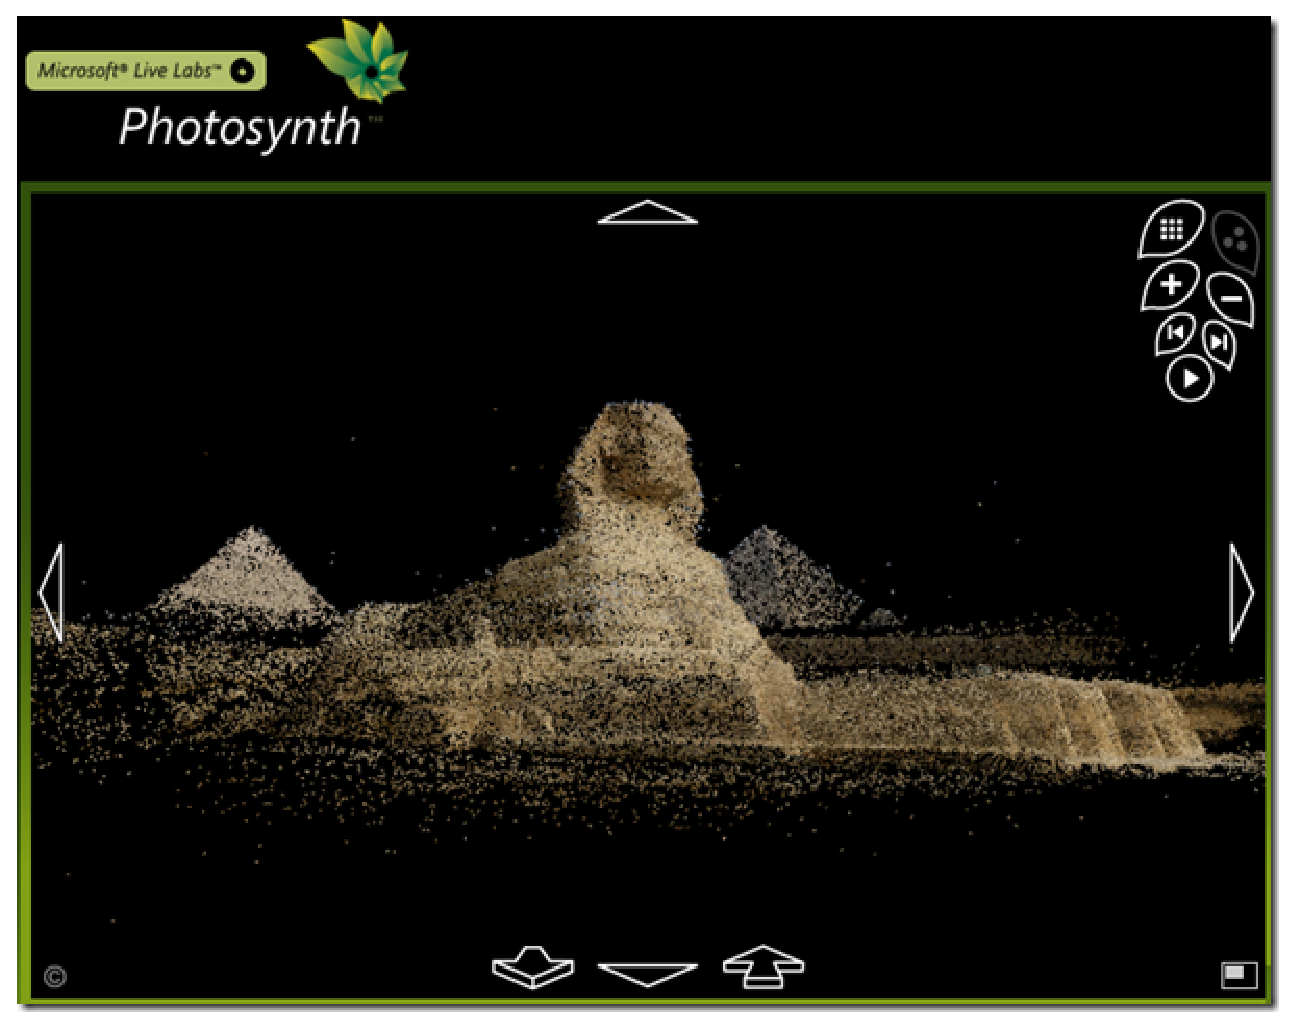
\includegraphics[width=250px]{photosynth}
  \end{center}
  \caption{An Egyptian Sphinx, viewed as Photosynth's point cloud \protect \cite**{photosynth}}
  \label{photosynthcloud}
\end{figure}

\begin{figure}
  \begin{center}
    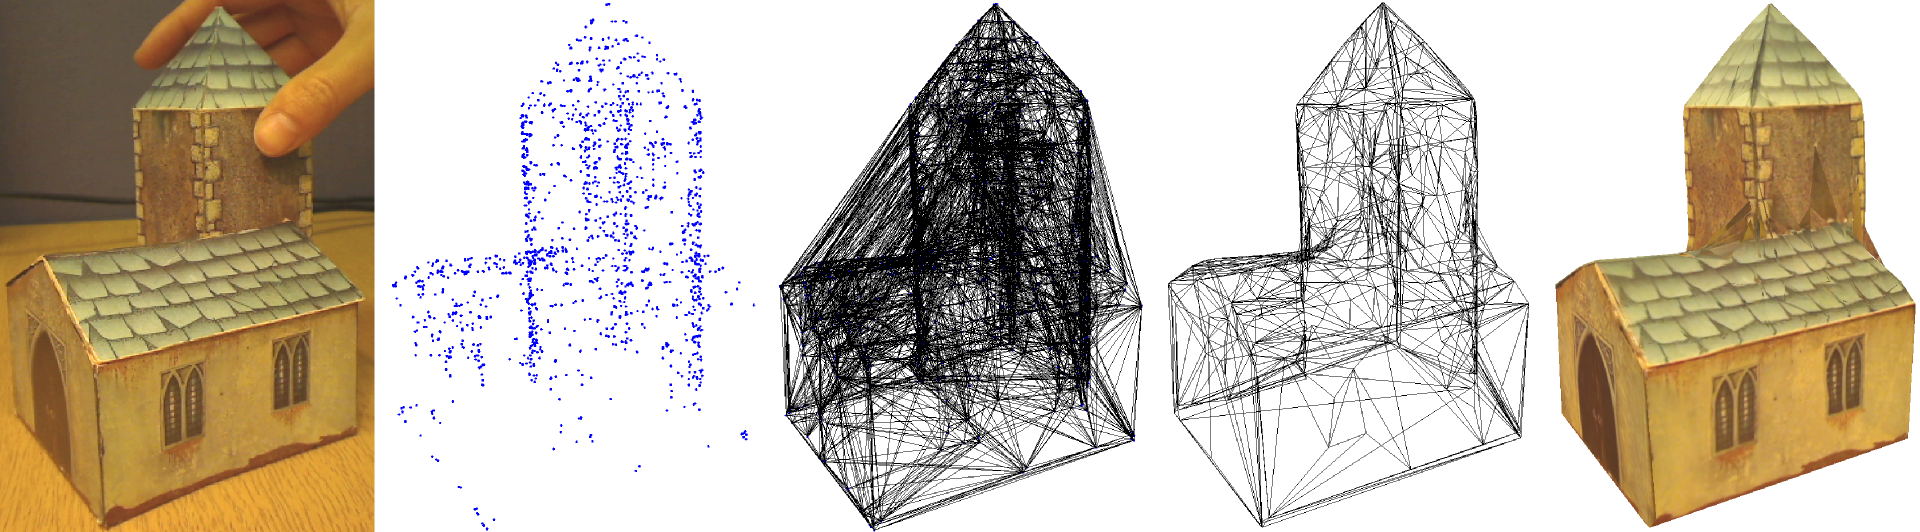
\includegraphics[width=340px]{proforma}
  \end{center}
  \caption{The stages of ProFORMA's automated modelling process \protect \cite**{proforma}}
  \label{proformaeg}
\end{figure}

Alternative approaches go to the other extreme: complete on-line processing of visual data, aiming for an interactive experience \cite**{proforma}. In ProFORMA, the application guides the user as to which areas of the target object it requires further data on, and shows the model in augmented reality as the scanning takes place. The approach taken by Pan is to perform structure-from-motion analysis on the rotating object in order to inform the application as to the angle at which it is viewing the object. From this, it generates and maintains a 3D point-map of the target object. This point map is used as input to a Delaunay Tetrahedralisation \cite**{dtet} process, which is then probabilistically carved to produce a complete mesh. Finally, texture is extracted from the video stream to suit the polygons of this mesh (see Figure~\ref{proformaeg} for an example). However, as we can clearly see in this example (of Qi Pan's own production!), the carving is imperfect; the modelled shape clearly does not quite match the input object, and extra polygons can be seen protruding from the surface of the bell-tower. Should a user wish to clean this up, they would first have to import the data into a 3D modelling package, and then attempt to understand the automated mesh that was generated, in order to alter the polygon geometry and remove these spurious constructions. Furthermore, they would have to manually modify the texture map, since ProFORMA has extracted texture for regions which do not exist in the source shape. 

Debevec et al. \cite**{architecture} produced an interesting, and similar, approach based on a series of static images and minimal user input, tailored primarily for architectural modelling. This required altogether less user input - simply marking edges on the images - but on its relatively limited test domain produced some strong results.

\begin{figure}
  \begin{center}
    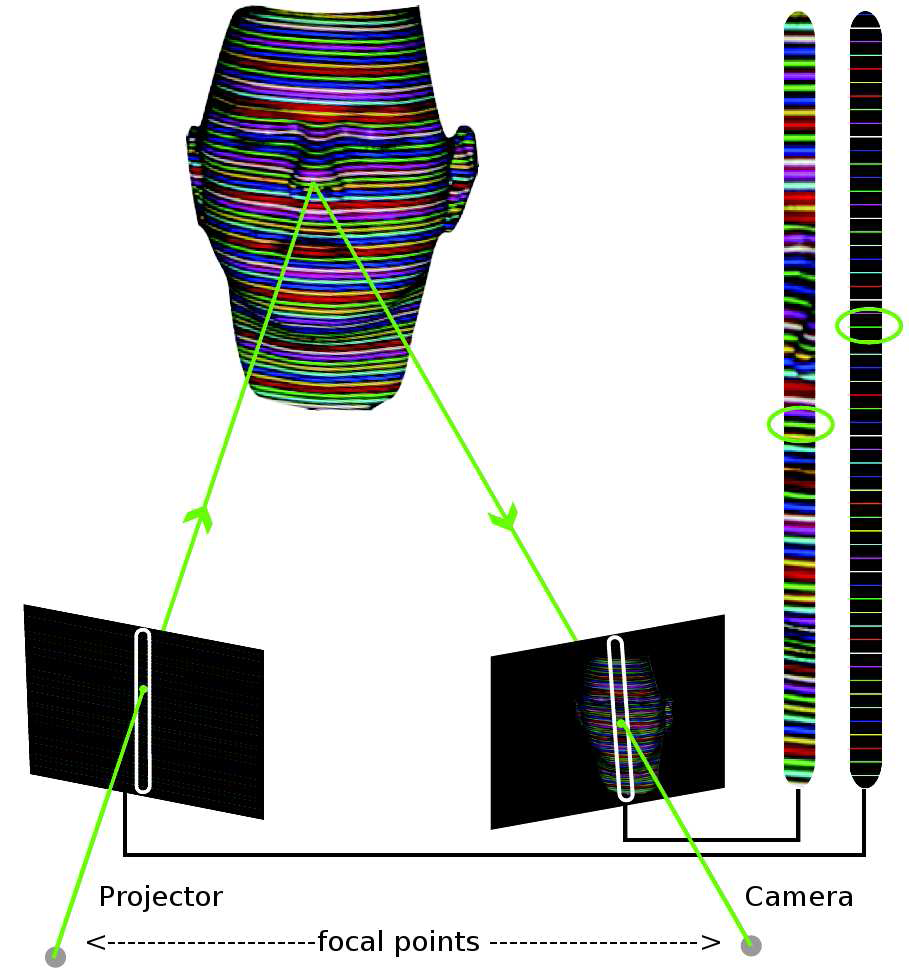
\includegraphics[width=300px]{lightproj}
  \end{center}
  \caption{An example of point projection from the human face using structured light \protect \cite**{lightface}}
  \label{faciallightpoint}
\end{figure}

Another approach that has received recent attention is Structured Light \cite**{structlight}. This entails controlling the lighting of the target object in such a way as to extract 3D data; it requires more equipment and a controlled environment, but can produce interactive performance. Typically, a known pattern of light (potentially changing over time) is projected onto the image, from a fixed source. A single lens may then pick up the way the pattern has fallen on the image, and use this to infer its 3D shape. The suitability of such a process for high-resolution complex modelling has already been shown with 3D facial scanning \cite**{lightface}, as in Figure~\ref{faciallightpoint}. 

\begin{figure}
  \begin{center}
    
\includegraphics[width=340px]{natal}
  \end{center}
  \caption{An example of how Project Natal projects a noisy depth-map onto the human skeleton, \copyright 2009 Microsoft}
  \label{natal}
\end{figure}

This approach is favoured by Microsoft, in their new ``Project Natal" motion camera, which exemplifies structured light's suitability for real-time processing. The Natal system gets around problems inherent in controlling the light in an environment by utilising an infra-red spectrum projection and camera - thereby also preventing visible projected light from dazzling the user. However, such an approach offers insufficient resolution for full 3D reconstruction; Natal extracts a depth map from the scene, and is primarily focused on using this for skeletal mapping and recognition (see Figure~\ref{natal}). Other structured light solutions may be more suitable for the problem described here, however the extra hardware and controlled environment required preclude it as an approach, based on the goals laid out for this system.

\subsection{Surface Reconstruction}

A common aspect of many of these systems is the need to construct a polygon mesh from a point cloud in an automated fashion. This problem is orthogonal to that of extracting the point cloud in the first place; many of these systems could use the same approaches, and differ only in the state-of-the-art at the time of their development. We have already mentioned Delaunay Tetrahedralisation, in the context of ProFORMA. However, this is not the only approach available.

\begin{figure}
  \begin{center}
    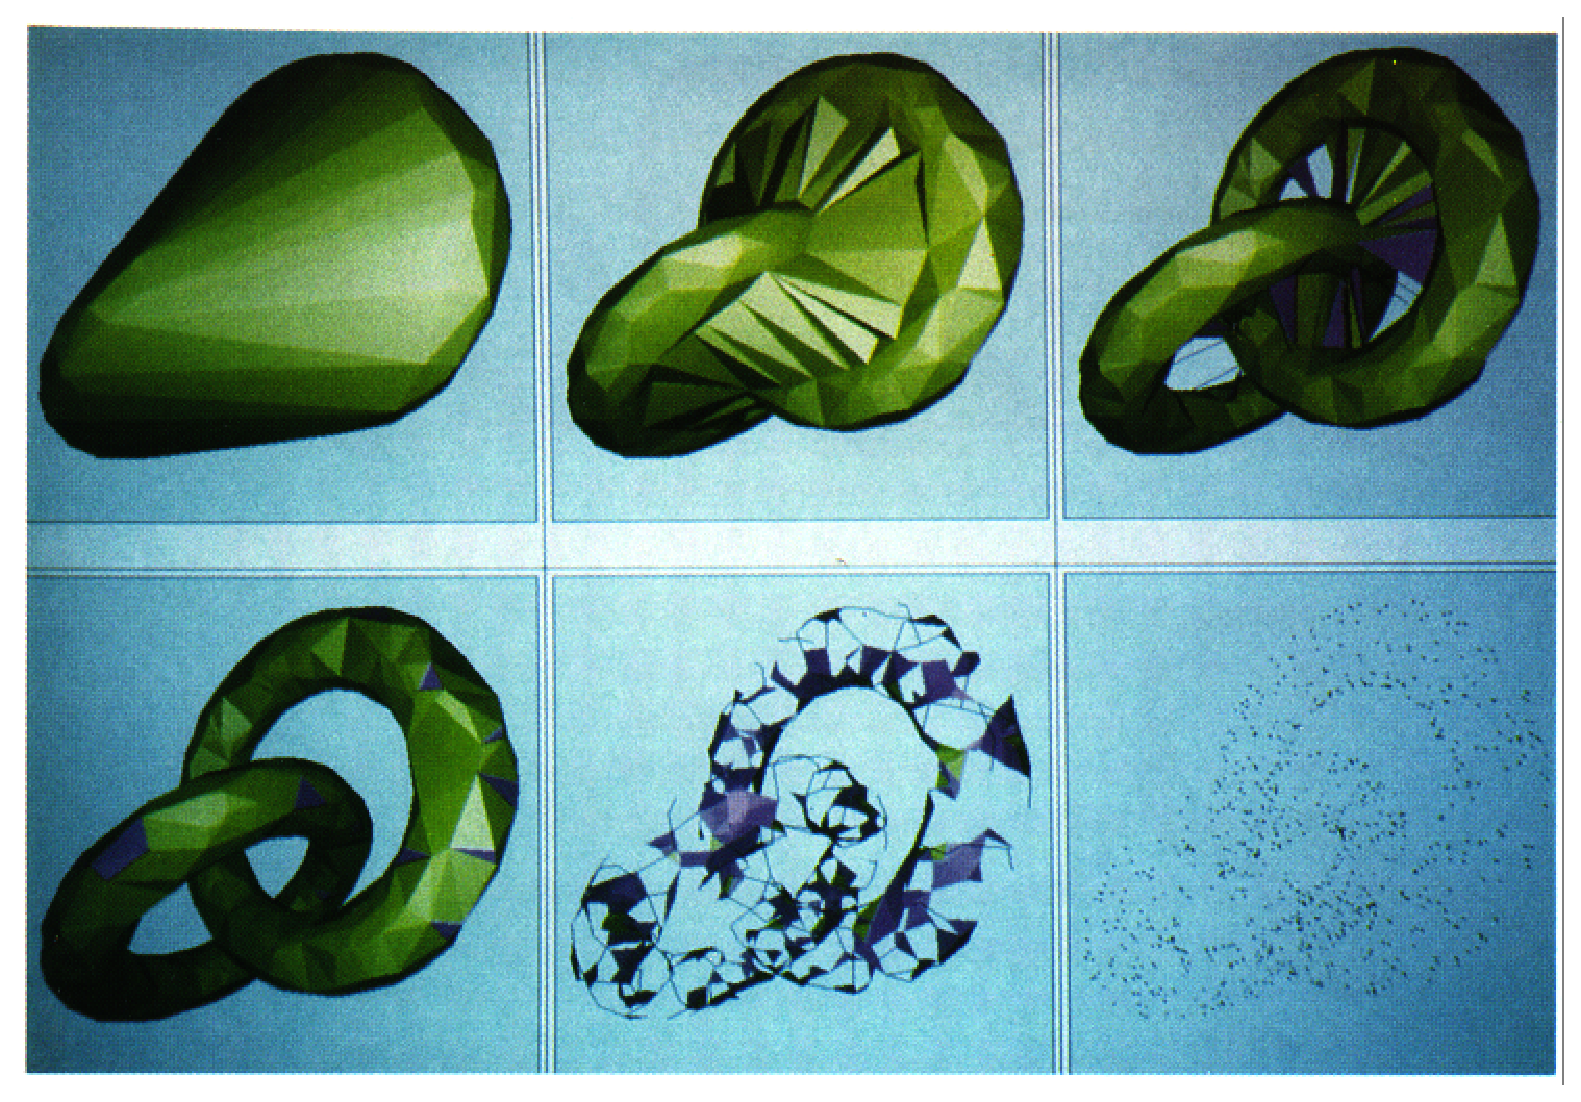
\includegraphics[width=340px]{alphashapes}
  \end{center}
  \caption{A progression of $\alpha$-shapes, with $\alpha$ ranging from $\infty$ to 0 left-to-right and top-to-bottom \protect \cite**{alpha}}
  \label{alphashapes}
\end{figure}

The notion of 3-dimensional $\alpha$-shapes \cite**{alpha} were introduced as an early attempt to fit a manifold onto a cloud of points in 3D space, based on Dalaunay Triangulation (and their dual, Voronoi diagrams). These shapes are a mathematically rigorous generalisation of the convex hull approach \cite**{hull}, with an additional parameter (the eponymous $\alpha$), which defines the range of the family of shapes; as $\alpha$ tends towards 0, the shape tends towards the point cloud. As $\alpha$ tends towards $\infty$, the shape tends towards the convex hull; for values in between, the shape is somewhere between the point cloud and the convex hull - it is not guaranteed that this $\alpha$-shape is fully connected, or necessarily convex, as the convex hull must be. See Figure~\ref{alphashapes} for an example of this in two disconnected tori.

An alternate approach is that of implicit surface reconstruction \cite**{unorgsurf,surface}, in which the surface is estimated as a \textit{simplicial surface} (a linear surface with triangular faces) based on the signed distance between it and the points that comprise its cloud. At each point, a tangent plane is defined as a linear approximation to the surface at that point - how to define the orientation of the planes is characterised by the author as one of the most challenging aspects of this approach. This is done by fitting the least-squares best fitting plane to those points in the ``neighbourhood" of the current point, and subsequently flipping planes to ensure that normals for sufficiently geometrically close points are pointing in similar directions. With these tangent planes constructed, the signed distance function can be estimated based on projecting points onto their nearest tangent plane. Finally, Hoppe uses a marching cubes algorithm \cite**{cubes} to trace contours and perform his final surface construction.

\subsection{User-Driven Vision-Augmented Reconstruction}

\begin{figure}
  \begin{center}
    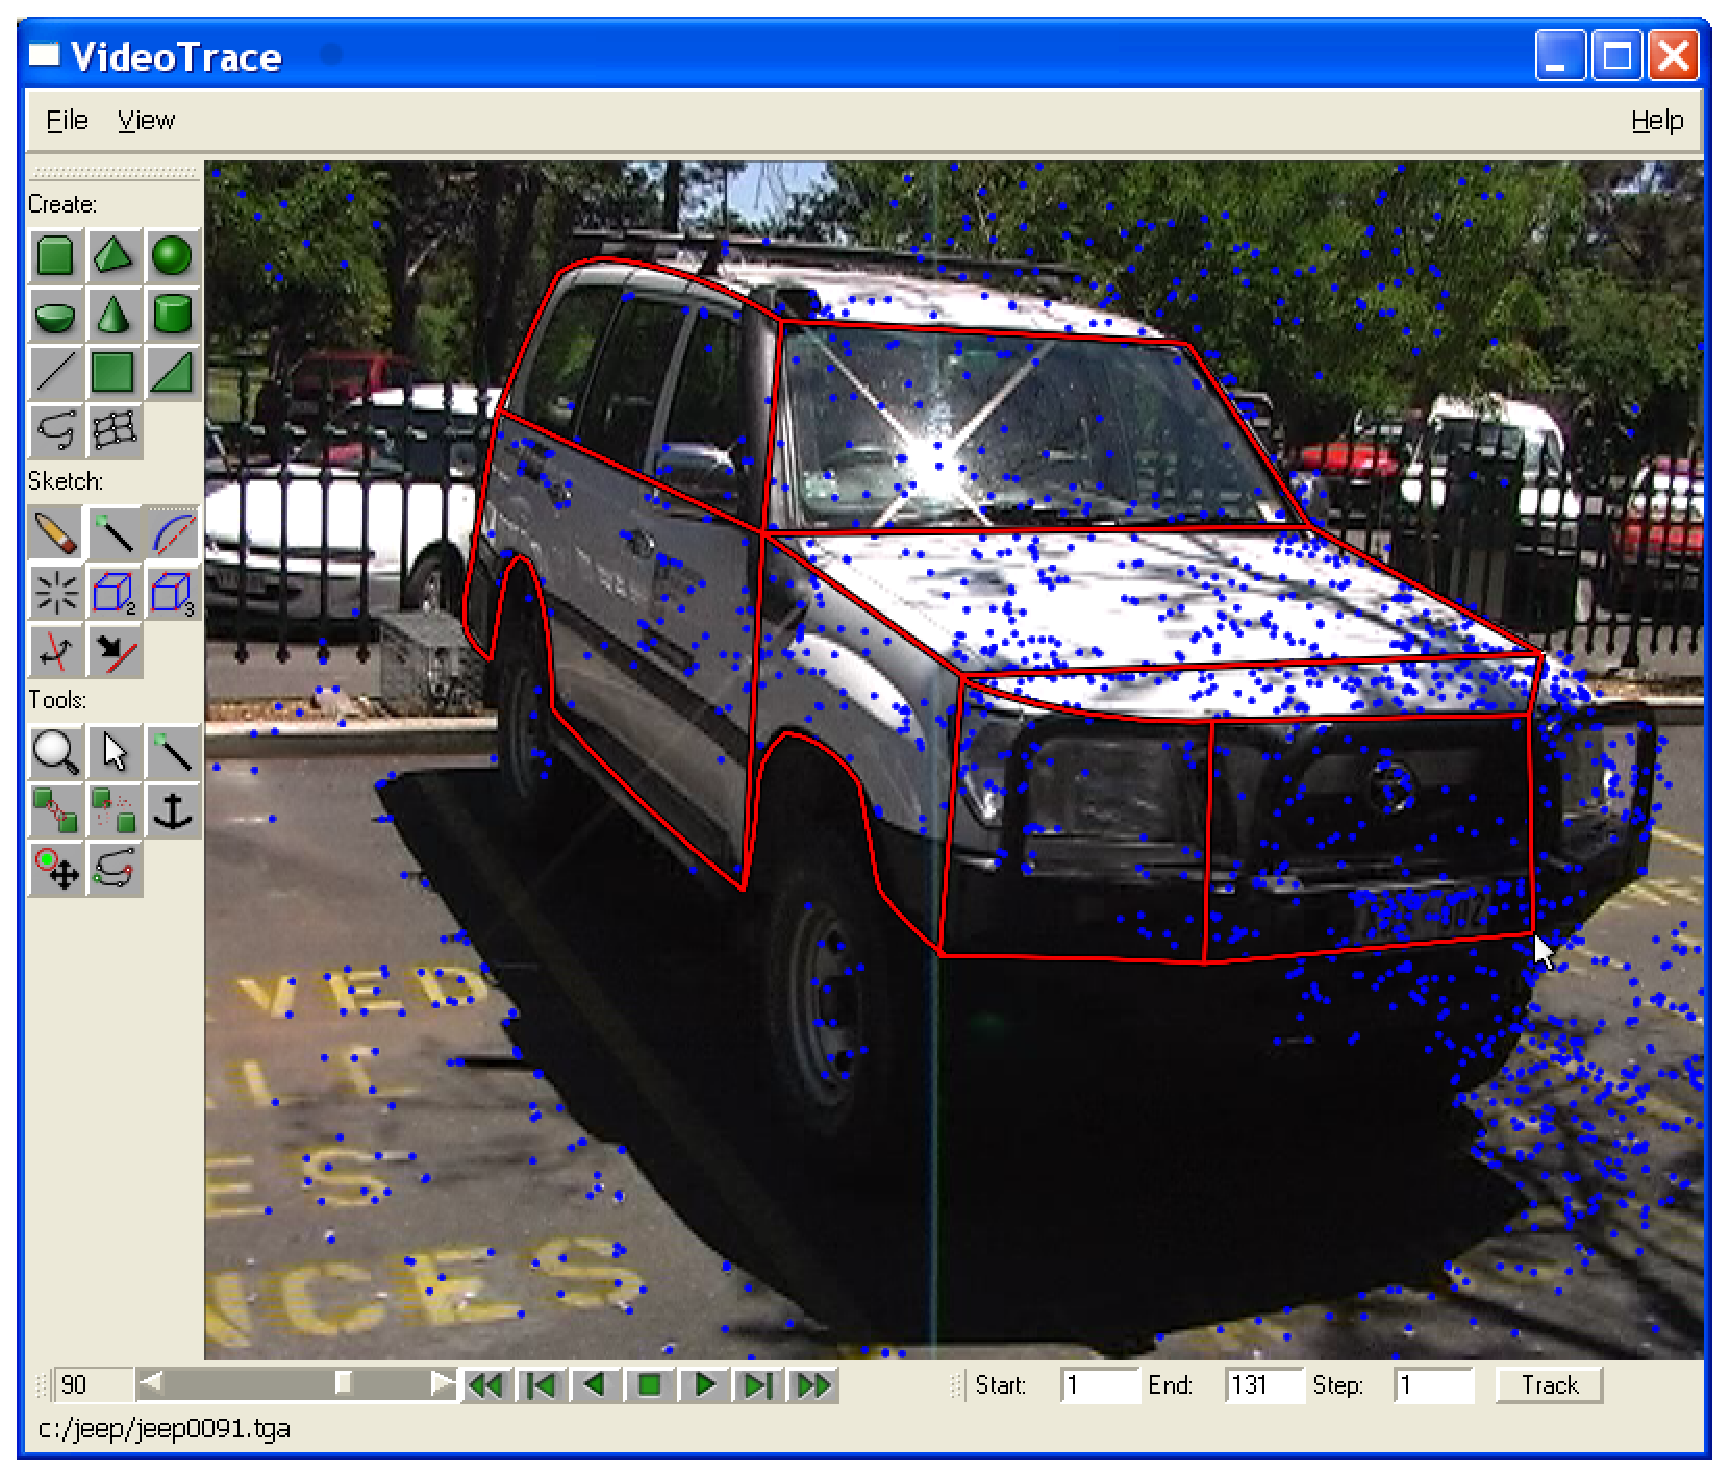
\includegraphics[width=340px]{videotrace}
  \end{center}
  \caption{An example of the VideoTrace User Interface in action \protect \cite**{videotrace}}
  \label{videotraceeg}
\end{figure}

The final approach we will examine is that taken by the likes of VideoTrace \cite**{videotrace}. These approaches recognise the difficulty inherent in producing a solution that will work for ``all of the people, all of the time", and instead focus on creating a toolkit that can be used to trivially craft a model from some video input.

VideoTrace (Figure~\ref{videotraceeg}) uses pre-recorded footage as input to structure from motion analysis, and extracts (in a pre-processing step) a 3D point cloud across the field of view of the camera throughout the sequence. At this time, it caches the results of a number of other computationally expensive vision tasks, such as superpixel segmentation, and thus edgelet delineation (along the boundaries of superpixels). Once this is complete, it presents a highly simplified modelling interface, not entirely dissimilar to SketchUp \cite**{sketchup}. 

VideoTrace uses the vision data already calculated to augment the user's ``tracing" of the video; the user is encouraged to ``scrub" the timeline back and forth, freezing the video on a given frame and then tracing shapes with the given tools (for example straight lines, free-hand drawing, and NURBS curves). As the user does this, VideoTrace snaps these lines to the nearest edgelets, permitting the user's inaccurate interactions to be enhanced by visual structure in the image. VideoTrace offers a suite of tools to help model occluded portions of objects too; for example, by extruding an existing shape or by mirroring geometry along a given plane. All of this processing is informed by visual cues in the image; for example, a user may draw the line of symmetry directly onto a frame of video, and VideoTrace will project that onto its geometry model and construct a fairly accurate mirroring plane. Finally, once the user moves from a given frame of video, VideoTrace processes the traced geometry once more, in order to fix perspective-related inaccuracies; using the continuity of frames to fit the trace to the edgelets in the video, continually enhancing its accuracy.

One obvious pitfall to a VideoTrace-style approach is that one must have enough recorded footage of the object to be modelled a priori; if the available footage doesn't quite show a part of the model, or the texture is occluded or in shadow, new video must be recorded - and this can't be known until one attempts the modelling process. By contrast, interactive systems using live video can show the user in real time what information is lacking, and how they should perhaps tweak their environment to obtain better results.

\subsection{Texture Extraction}

\begin{figure}
  \begin{center}
    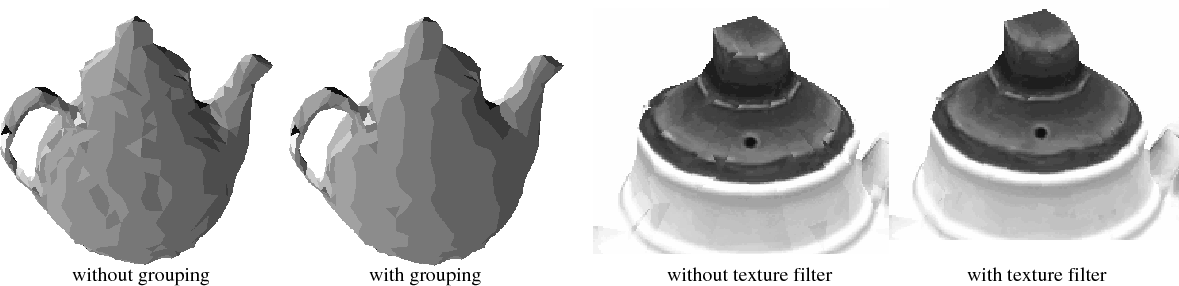
\includegraphics[width=340px]{texture}
  \end{center}
  \caption{A comparison of the various stages of multi-view texture extraction \protect \cite**{texmultiview}}
  \label{texture}
\end{figure}

The final key aspect of these approaches we have not studied in detail is the problem of extracting texture from the input video, and mapping that onto the output geometry. There are a number of elements to this; selection of video frames for texture, compensation for lens distortion and projection of the texture into 2D space, and mapping of this texture onto the generated model such that it forms a contiguous view. A popular technique is to use texture from multiple camera views \cite**{texmultiview} in order to minimise distortions at the boundaries. The approach outlined by Niem and Broszio requires calibration of the camera \cite**{camcalib} in order to remove distortion and reduce aberrations in the input image due to lens shape. It assigns triangles on the surface of the mesh a camera image (selected according to best resolution). Groups of triangles which are textured by the same image (within some tolerance) are then considered to be \textit{surface regions}. These regions are refined so as to group them together as much as possible, reducing the number of region boundaries. Finally, it filters textures at the boundaries by linearly interpolating the texture from one view to the other across the boundary edge. The result is a smoothly varying texture over the surface of the shape; however, it does necessitate choosing sub-optimal video frames for some polygons in the texture-map. The end result of this is a texture map which requires less space to store, and varies smoothly, and thus the trade-off is probably acceptable. Niem and Broszio also describe a technique for synthesising texture for polygons which lack information, by reflecting texture from adjacent regions and blending the results.

The approach taken by Debevec et al. (1996, discussed earlier) sidesteps the issues around perspective quite neatly; the interactive output of their system dynamically selected the texture frame to use based on the current position of the camera. Their approach uses a similar blend technique at polygon boundaries, to reduce rendering artefacts. What is not made immediately clear is how this technique handles a smoothly changing camera; whether it sticks with what is potentially a later non-ideal texture, blends between two target textures smoothly (the problem of knowing which texture to blend \textit{to} seems non-trivial, as it involves predicting the user's interactions), or simply ``jumps" from one texture frame to another at some point in the interaction is not made clear.

\begin{figure}
  \begin{center}
    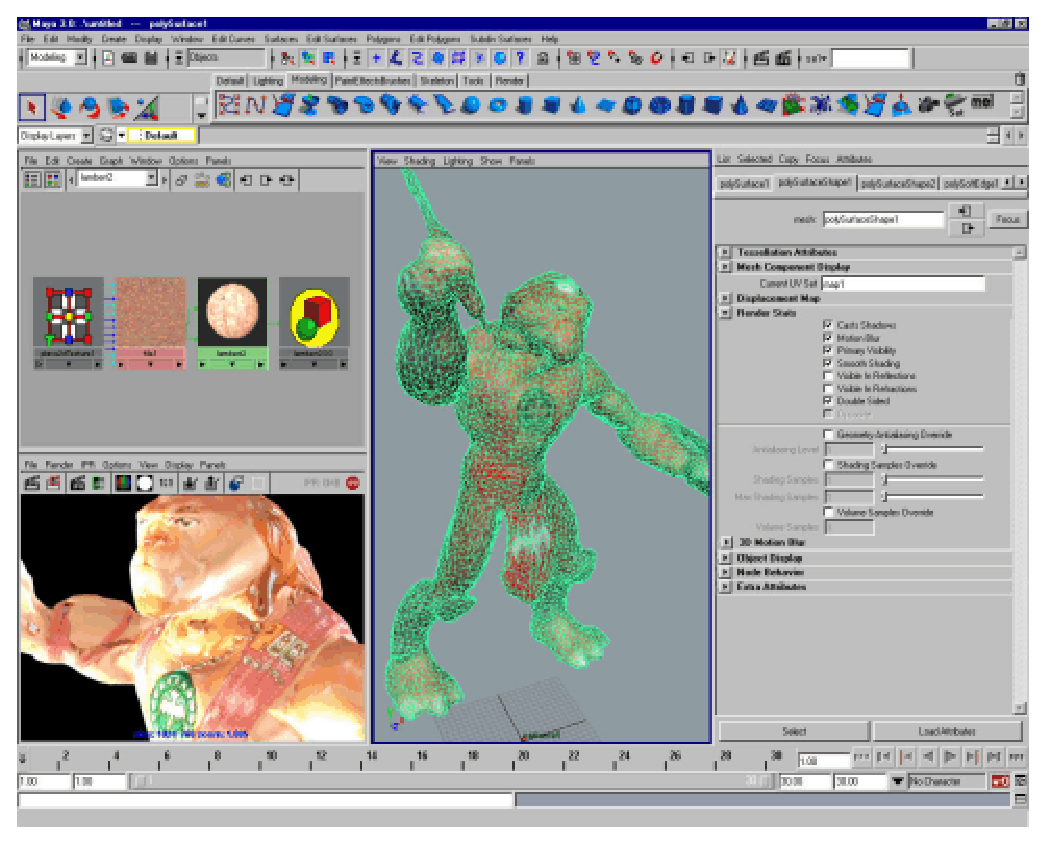
\includegraphics[width=340px]{maya}
  \end{center}
  \caption{An example of Maya's complex user interface (autodesk.com, 2009)}
  \label{maya}
\end{figure}

\section{Approach}
\subsection{Overview}

\begin{wrapfigure}{r}{80pt}
  \vspace{-37pt}
  \begin{center}
    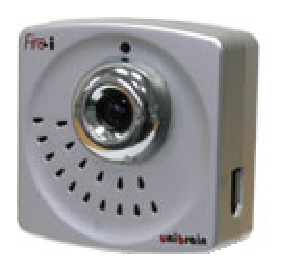
\includegraphics[width=80pt]{firei}
  \end{center}
  \vspace{-20pt}
  \caption{A Unibrain Fire-i\texttrademark}
  \label{firei}
  \vspace{-15pt}
\end{wrapfigure}

Broadly speaking, the approach described herein is to carefully delineate responsibilities between human and machine, so as to make the best possible use of their own varieties of intelligence. For example, heavy \textit{mathematical} reconstruction is an ideal problem domain for a computer; whereas more \textit{interpretive} problems are better solved by the human. The goal of this system is to minimise the complexity of user input (in particular when compared to the likes of Autodesk Maya, Figure~\ref{maya}) by augmenting it with vision technologies. The primary input device is to be a single-lensed commodity webcam, such as the Unibrain Fire-i\texttrademark ~seen in Figure~\ref{firei}.

The goal of the system is to permit the user to move the webcam in space around the object they wish to ``scan", and identify key features to the scanner. Throughout this process, the model created will be updated and continually shown as an augmented reality overlay, so that the user may easily tweak the result and examine its accuracy; this continual feedback loop is required to make the most of the interactivity of the system.

\subsection{Ego-Motion Recovery}
The first problem to be considered in relation to this solution is that of working out where in space the camera is located, and directed, at any given time. Some augmented reality systems, such as Layar, do this by using positioning sensors like GPS in tandem with a magnetometer for orientation. This is a relatively simple way of performing approximate localisation, however the problem of scale rapidly arises; if you desire a resolution of greater than approximately one meter, GPS will quickly fail you. Thus, whilst well suited to (for example) modelling the layout of a whole city, it is less suitable for a user wishing to record a detailed scan of an object on their desk. 3rd party \textit{local} positioning systems operate on a similar principle to GPS, and can provide much greater resolution over small areas. However, they are expensive and seem an unnecessary extra burden for the user to own and maintain. Ideally, the ego-motion recovery problem should be solved without the application of further hardware.

Systems like VideoTrace \cite**{videotrace} are able to make use of processor-intensive offline tracking applications  to perform camera motion recovery - in the case of VideoTrace, the Voodoo Camera Tracker \cite**{voodoo}. These are commonly used in the visual effects industry as well, and thus much effort has gone into research and development on these. They tend to produce excellent and smooth results, even to the extent of being able to automatically fix operator-induced visual defects such as camera shake. However, their processing is designed for batch runs on high-performance machines; they are wholly insuitable to a real-time processing application.

To this end, a number of computer vision researchers have worked on solving the problem of real-time \textit{monocular SLAM}; \textit{S}imultaneous \textit{L}ocalisation \textit{A}nd \textit{M}apping using a single camera lens, with high enough throughput to be used as part of a larger real-time system \cite**{slam}. In essence, a SLAM system works by estimating the movement of the camera between frames based on the motion of the intersection-set of detected feature points in each frame. This approach can produce very accurate results, assuming non-degenerate camera motion. There are instances in which a SLAM-based system can get ``confused", however; it is important that the localiser can detect these cases and re-localise based on the presented frame

\begin{figure}
  \begin{center}
    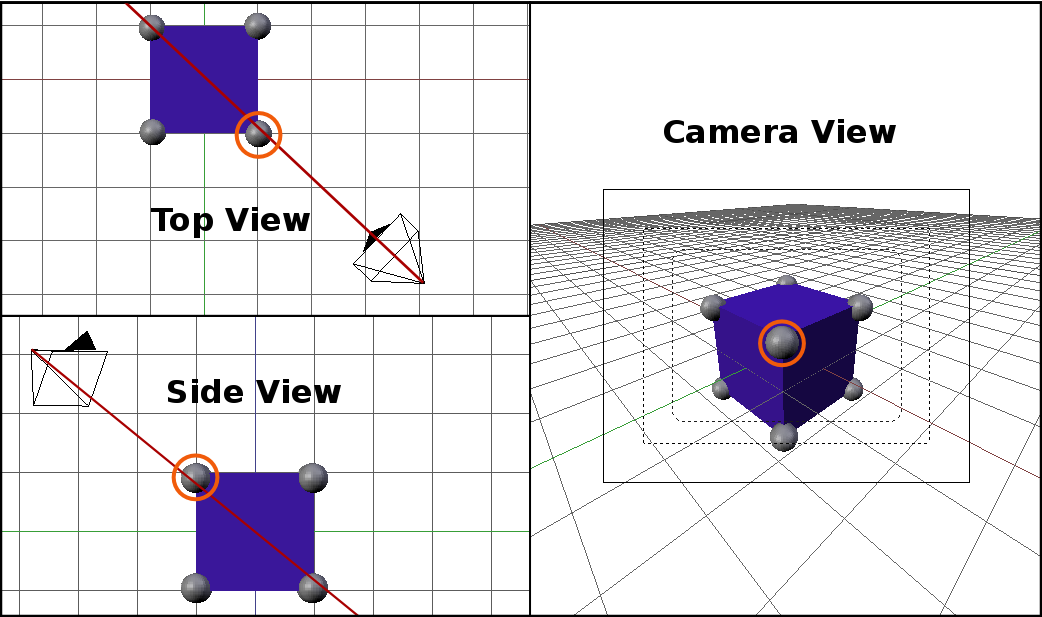
\includegraphics[width=340px]{cameraaim}
  \end{center}
  \caption{An example of the look-vector of the camera aiming towards a set of candidate feature points (marked as spheres), with the closest to that vector ringed}
  \label{lookvec}
\end{figure}

A recent development on existing SLAM approaches is PTAM; \textit{P}arallel \textit{T}racking \textit{A}nd \textit{M}apping \cite**{ptam}. PTAM improves the robustness of SLAM by using a faster approach to motion estimation, thus allowing it to consider far more points in a given iteration of recognition. It can maintain its 3D point-map in a separate thread to the actual motion processing, further reducing the overhead in the tracking thread - making excellent use of common multi-core processing systems available in desktop and laptop computers today. PTAM requires a stereo initialisation at the start, but once this has been processed it will provide a reliable transformation to describe the translation and orientation of the camera in 3D space, relative to an arbitrary zero-point, on an arbitrary scale (both of which are constructed relative to the position and motion of the camera during stereo initialisation). As an added benefit, PTAM maintains a map of the features it recognises in 3D-space. It is highly challenging, given only the position and orientation of the camera, to determine precisely what point in space the user is attempting to point to; there are insufficient bounds on the problem, rendering the system with an infinite vector of possible points. This PTAM point-map can be used to augment such decisions, by deciding which point in the map is closest to the camera's look-vector (see Figure~\ref{lookvec}).

PTAM (as with many SLAM systems) works best with camera lenses exhibiting a wide field-of-view; in this way, it can gather even more points with which to localise. However, this does mean that the images provided to the processing system are distorted by the wide angle lens. In order to account for this, PTAM requires a one-time camera calibration process, which feeds the parameters on its ATAN-Camera model \cite**{atancam}. It is therefore important that, when considering the user interface, this distortion is also considered.

\subsection{User Interface}
As already discussed, the primary user input is to be a simple webcam. This device is to be augmented with a maximum of two other digital inputs (i.e. buttons). These inputs could be positioned on the camera itself - indeed, some cameras already have these. However, in the interests of the most generally usable solution possible, these inputs will be assumed to be on the keyboard.

It is envisaged that the user would interact with the model on the basis of ``tools"; different processors to operate on the scene. One of these input buttons should interact with the selected tool, whilst the second is used to select the tool the user wishes to make use of. Potential examples of tools might be to move points in space, to bisect an edge, or to delete a given vertex in the model.

Feedback is to be provided to the user on a continuous basis. Using the tracking information from PTAM, as well as its camera calibration data, it is possible to project a 3D render of the current model on top of the current camera frame such that it provides a perspective-correct overlay of the current model on the actual object being modelled. To get this right, it will be best to render the model at each stage relative to the co-ordinate system set up by PTAM, then use OpenGL's projection matrix to project those from 3D-space into camera-space. In this way, the projection may also be accelerated by graphics hardware available on the user's computer. However, the scene will need to be rendered twice; once onto an alpha-channel framebuffer in order to do the projection from world-space into screen-space, and once from that onto the camera frame to take into account camera lens distortion. In this manner, an accurate augmented reality scene will be projected atop the camera's image, permitting the user to visualise and improve their results throughout the modelling process.

\subsection{Modelling}
\label{approachmodel}
The modelling process itself should be as general as possible; models should consist of triangular polygons assembled into a valid 3D model. As far as possible, problems such as degenerate faces, co-occurrent points, isolated vertices, etc should be avoided. It is not \textit{necessary} that the produced model be a closed hull; but it should be \textit{possible} to create such a model with this system. The precise details of the modelling process are open to experiments in user-interface design, however it is expected to be a gradual process. The user should work in one of two ways; either they identify vertices in space, and connect them to make the faces of their model, or they may place ``primitives" in the scene (such as planes, cubes, and the like) and manipulate them to best fit the model. Furthermore, there may be cases where a hybrid approach is needed - the user may construct an initial shape that approximates their model, and then refine it over time to improve its accuracy.

It should be possible for the system to use some of the vision techniques above to improve its results - for example, texture extraction may be fully automated. It is important that any vision techniques that are used do not interfere with the will of the user; it must be possible to override their results. A likely example is that of vertex positioning - augmenting the user's input with information about features in the scene can make the task of placing points in 3D space much easier. However, the user \textit{must} have the option of placing points at features that are not detected by vision algorithms. Another useful example of where vision techniques may enhance the modelling process is in edge-fitting; if the user joins two vertices, and the edge is found to run along an edge in the image, the edge that is created in the model may, perhaps, insert extra points in order to better follow the contours of the image. The precise vision techniques that may be applied should be investigated and evaluated for their validity and utility in their particular use cases.

\section{Implementation}
\subsection{Architecture}

\begin{figure}
  \begin{center}
	\scalefont{0.9}
	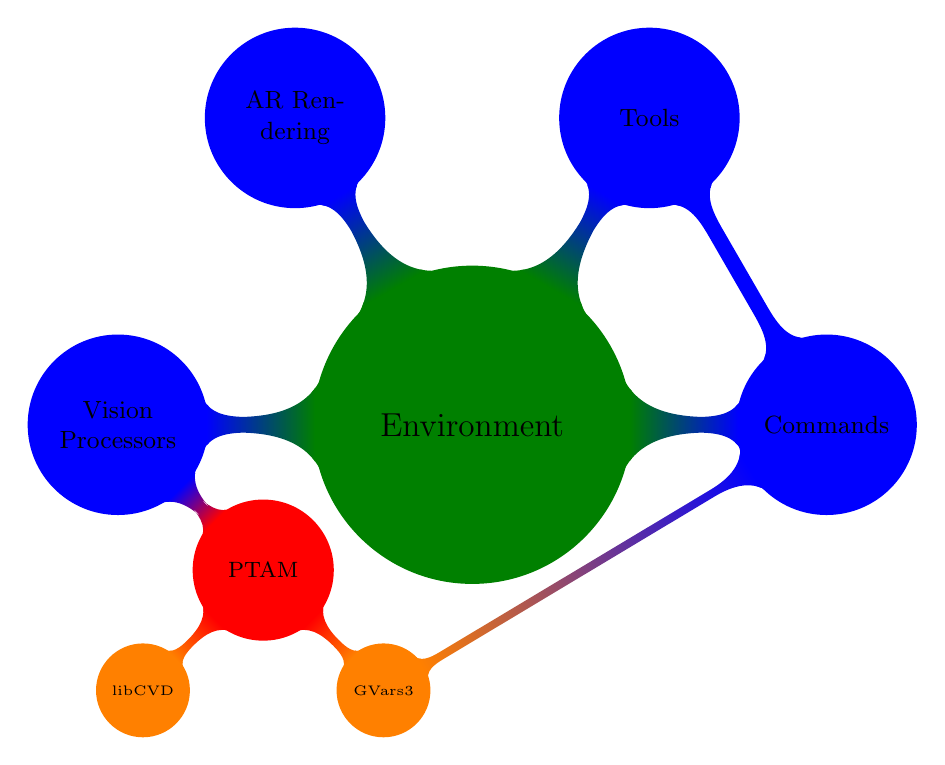
\begin{tikzpicture}[scale=0.9]
  	  \path[mindmap,concept color=green!50!black,text=black]
	    node[concept] {Environment}
	    [clockwise from=180]
	    child[concept color=blue] {
	      node[concept] (proc) {Vision Processors} 
	      [clockwise from=-45]  
	      child[concept color=red] {
	        node [concept] {PTAM}
	        [clockwise from=-45]
	        child[concept color=orange] {
	          node[concept] (gvar) {GVars3} 
	        }
	        child[concept color=orange,sibling angle=90] { 
	          node[concept] (cvd) {libCVD} 
	        }
	      }
	    }  
	    child[concept color=blue] {
	      node[concept] (ren) {AR Rendering}
	    }
	    child[concept color=blue] {
	      node[concept] (tool) {Tools}
	    }
	    child[concept color=blue] {
	      node[concept] (cmd) {Commands}
	    };
	  \path (cmd) to[circle connection bar switch color=from (blue) to (orange)] (gvar);
	  \path (tool) to[circle connection bar switch color=from (blue) to (blue)] (cmd);
	\end{tikzpicture}
	\normalsize
  \end{center}
  \caption{Architectural Plan}
  \label{archmindmap}
\end{figure}


\subsection{Model}

\begin{figure}
  \begin{center}
	\scalefont{0.75}
	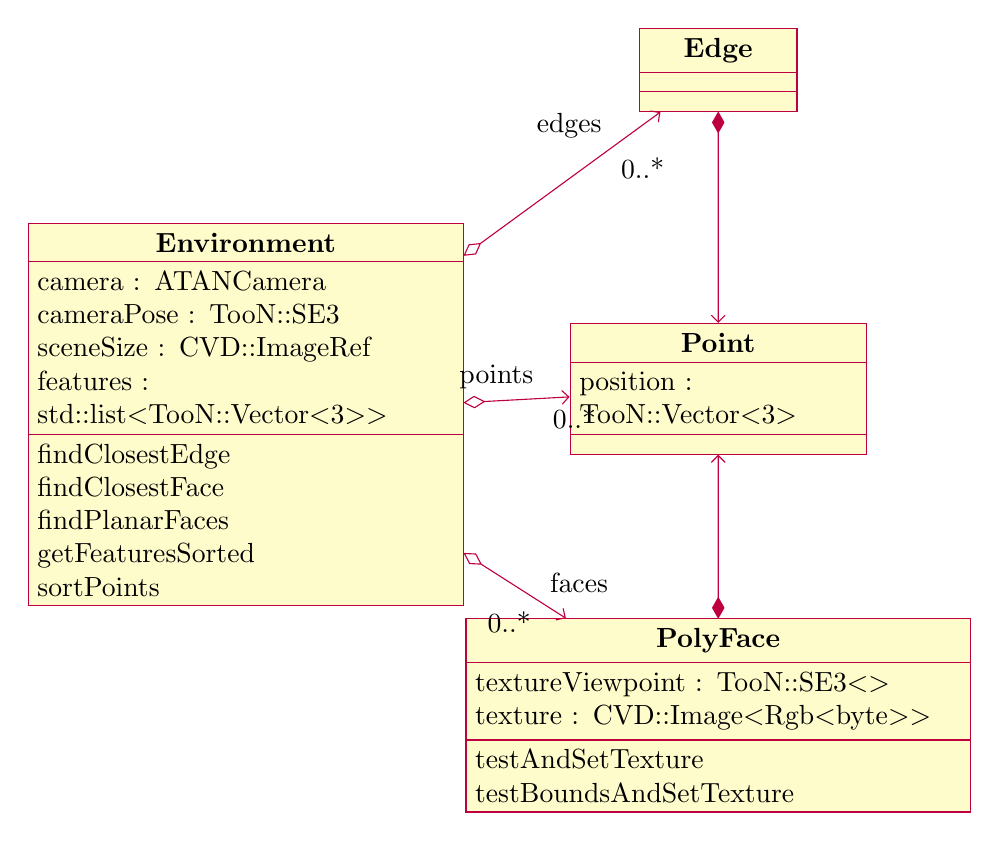
\begin{tikzpicture}[scale=0.75]
	  \begin{class}[text width=150px]{Environment}{0,1.7}
            \attribute{camera : ATANCamera}
	    \attribute{cameraPose : TooN::SE3}
	    \attribute{sceneSize : CVD::ImageRef}
	    \attribute{features : std::list\textless TooN::Vector\textless 3\textgreater\textgreater }
	    
	    \operation{findClosestEdge}
	    \operation{findClosestFace}
	    \operation{findPlanarFaces}
	    \operation{getFeaturesSorted}
	    \operation{sortPoints}
  	  \end{class}

  	  \begin{class}[text width=175px]{PolyFace}{8,-5}
	    \attribute{textureViewpoint : TooN::SE3\textless \textgreater }
	    \attribute{texture : CVD::Image\textless Rgb\textless byte\textgreater \textgreater }
	    
	    \operation{testAndSetTexture}
	    \operation{testBoundsAndSetTexture}
	  \end{class}

	  \begin{class}[text width=100px]{Point}{8,0}
	    \attribute{position : TooN::Vector\textless 3\textgreater}
	  \end{class}

	  \begin{class}[text width=50px]{Edge}{8,5}
	  \end{class}
	  
	  \aggregation{Environment}{faces}{0..*}{PolyFace}
	  \aggregation{Environment}{edges}{0..*}{Edge}
	  \aggregation{Environment}{points}{0..*}{Point}
	  
	  \composition{Edge}{}{}{Point}
	  \composition{PolyFace}{}{}{Point}
	  
	\end{tikzpicture}
	\normalsize
  \end{center}
  \caption{Model Class Diagram}
  \label{modelclasses}
\end{figure}

\subsection{Augmented Reality Rendering \& User Experience}

\subsection{Plugins}
\begin{figure}
  \begin{center}
        \scalefont{0.75}
        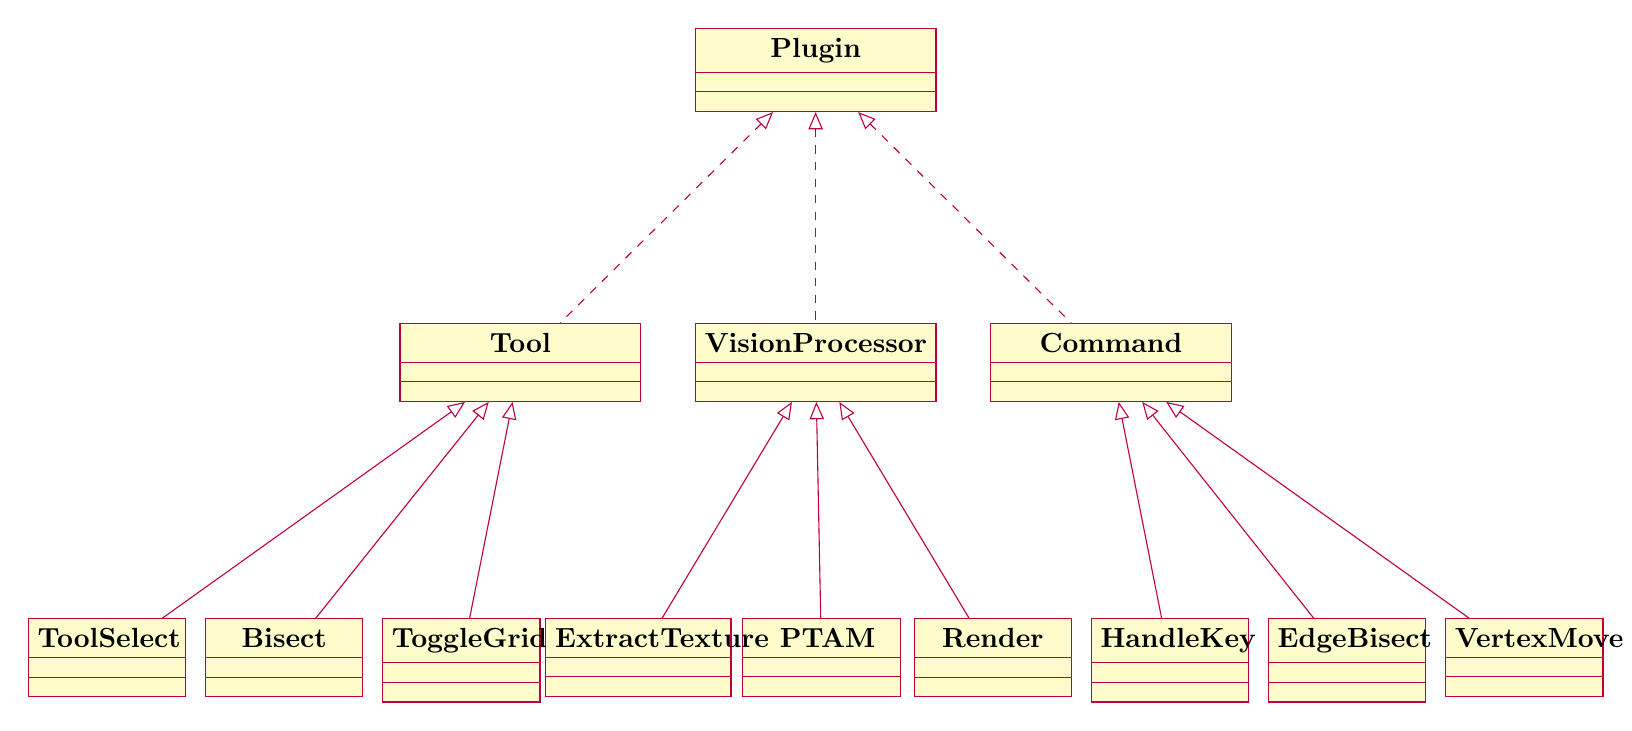
\begin{tikzpicture}[scale=0.75]
          \begin{class}[text width=80px]{Plugin}{0,0}
          \end{class}

          \begin{class}[text width=80px]{VisionProcessor}{0,-5}
            \implement{Plugin}
          \end{class}

          \begin{class}[text width=30px]{PTAM}{0.1,-10}
            \inherit{VisionProcessor}
          \end{class}

          \begin{class}[text width=50px]{Render}{3,-10}
            \inherit{VisionProcessor}
          \end{class}

          \begin{class}[text width=60px]{ExtractTexture}{-3,-10}
            \inherit{VisionProcessor}
          \end{class}

          \begin{class}[text width=80px]{Command}{5,-5}
            \implement{Plugin}
          \end{class}

          \begin{class}[text width=50px]{HandleKey}{6,-10}
            \inherit{Command}
          \end{class}

          \begin{class}[text width=50px]{EdgeBisect}{9,-10}
            \inherit{Command}
          \end{class}

          \begin{class}[text width=50px]{VertexMove}{12,-10}
            \inherit{Command}
          \end{class}

          \begin{class}[text width=80px]{Tool}{-5,-5}
            \implement{Plugin}
          \end{class}

          \begin{class}[text width=50px]{ToolSelect}{-12,-10}
            \inherit{Tool}
          \end{class}

          \begin{class}[text width=50px]{Bisect}{-9,-10}
            \inherit{Tool}
          \end{class}

          \begin{class}[text width=50px]{ToggleGrid}{-6,-10}
            \inherit{Tool}
          \end{class}

        \end{tikzpicture}
        \normalsize
  \end{center}
  \caption{Plugin Class Diagram}
  \label{pluginclasses}
\end{figure}

\subsection{Vision Processors}

\subsection{Toolset}

\section{Evaluation}
In order to ascertain the extent to which the finished product meets these criteria, carefully defined evaluation must be undertaken. It is not sufficient that the system simply accomplishes the above goals - there must be a methodology defined to ascertain how \textit{well} it accomplishes those goals. Therefore, two different types of evaluation will be undertaken; end-to-end acceptance testing, and numerical analysis of the accuracy of the result.

\subsection{Acceptance Testing}
Acceptance testing should consist of attempting to model a collection of real-world objects, of varying complexity; for example, ranging from a book to a more complicated shape, such as a detailed model or a pair of shoes. If the finished product is capable, testing it on a variety of scales would be advantageous; say, the view from a balcony as well as the aforementioned articles. This model construction should take place in a noisy environment; with uncontrolled lighting, other objects in the area, and the like, in order to best simulate the environment in which the system is designed for use. 

Once the modelling of each of these has been completed, they should be exported to disk, and imported into a 3D package for further analysis and raytracing; thus demonstrating the suitability of the system for producing data of real use. If the 3D package supports model checking, these static checks should be run on the produced model to check for invalidities such as degenerate faces and isolated vertices (as discussed in Section~\ref{approachmodel}).
\pagebreak

\subsection{Accuracy}
The numerical analysis of the system's accuracy is altogether less straightforward, as there is no perfect ``gold standard" approach against which the final product can be measured. Furthermore, an artistic ``from scratch" model against which to compare would be both hard to find and not necessarily created with accuracy in mind. If the hardware were available, the geometry that the system outputs can be compared against the point-cloud generate by a LIDAR scanner. This has the distinct advantage of testing the geometry separately from the texture. To some extent, the correctness of texture mapping can be inspected visually; however, a numerical approach would be desirable. To this end, an approach which compares the augmented-reality frame and the source camera frame from a few different perspectives would test the accuracy of the complete system; geometry, texture mapping, AR rendering, and even camera calibration. Of course, this means that if any one of these is deficient then the whole system will be deemed inaccurate. The obvious way of doing that would be to simply compare the pixel values of the two frames in the framebuffer. This would provide a quick and easy way of telling how accurate the system is overall; the average percentage pixel difference across the entire image should give an index of accuracy. Another approach would be to perform feature detection on the source and AR camera frames, and estimate the motion of co-occurrent features between the two; any features that are not within the model would not have moved, but those which \textit{were} modelled, would be expected to exhibit some form of motion. 

\subsection{Usability}
A third factor that remains unmeasured is the extent to which a new user can pick up the software and learn to use it; one aspect of this is documentation, the other a highly qualitative ``user friendliness". This can hypothetically also be tested, by giving the system to a small cross-section of different users and observing how readily they learn to use it. Worthy of note here is the relative difficulty with which most users learn 3D packages, such as Maya or 3D Studio Max - most 3D tools are highly complex, with many months of learning curve. If a user can pick this system up and start using it to model and texture objects inside of an hour then it should rate quite highly on the usability scale!

\subsection{Summary}
Combining these three approaches it should be possible to give both a qualitative and quantitative analysis of the suitability of the solution for purpose. If it can complete the above tasks, be found to be of reasonable accuracy, and can be picked up by new users with relative ease, it will be deemed to be a success. 

\clearpage
\renewcommand*{\refname}{\section{References}}
\bibliography{Report}
\bibliographystyle{dcu}

\end{document}          
